\documentclass[11pt,a4paper]{report}
\usepackage[textwidth=37em,vmargin=30mm]{geometry}
\usepackage{calc,xunicode,amsmath,amssymb,paralist,enumitem,tabu,booktabs,datetime2,xeCJK,xeCJKfntef,listings}
\usepackage{tocloft,fancyhdr,tcolorbox,xcolor,graphicx,eso-pic,xltxtra,xelatexemoji}

\newcommand{\envyear}[0]{2025}
\newcommand{\envdatestr}[0]{2025-01-08}
\newcommand{\envfinaldir}[0]{webdb/2025/20250108/final}

\usepackage[hidelinks]{hyperref}
\hypersetup{
    colorlinks=false,
    pdfpagemode=FullScreen,
    pdftitle={Web Digest - \envdatestr}
}

\setlength{\cftbeforechapskip}{10pt}
\renewcommand{\cftchapfont}{\rmfamily\bfseries\large\raggedright}
\setlength{\cftbeforesecskip}{2pt}
\renewcommand{\cftsecfont}{\sffamily\small\raggedright}

\setdefaultleftmargin{2em}{2em}{1em}{1em}{1em}{1em}

\usepackage{xeCJK,xeCJKfntef}
\xeCJKsetup{PunctStyle=plain,RubberPunctSkip=false,CJKglue=\strut\hskip 0pt plus 0.1em minus 0.05em,CJKecglue=\strut\hskip 0.22em plus 0.2em}
\XeTeXlinebreaklocale "zh"
\XeTeXlinebreakskip = 0pt


\setmainfont{Brygada 1918}
\setromanfont{Brygada 1918}
\setsansfont{IBM Plex Sans}
\setmonofont{JetBrains Mono NL}
\setCJKmainfont{Noto Serif CJK SC}
\setCJKromanfont{Noto Serif CJK SC}
\setCJKsansfont{Noto Sans CJK SC}
\setCJKmonofont{Noto Sans CJK SC}

\setlength{\parindent}{0pt}
\setlength{\parskip}{8pt}
\linespread{1.15}

\lstset{
	basicstyle=\ttfamily\footnotesize,
	numbersep=5pt,
	backgroundcolor=\color{black!5},
	showspaces=false,
	showstringspaces=false,
	showtabs=false,
	tabsize=2,
	captionpos=b,
	breaklines=true,
	breakatwhitespace=true,
	breakautoindent=true,
	linewidth=\textwidth
}






\newcommand{\coverpic}[2]{
    % argv: itemurl, authorname
    Cover photo by #2~~(\href{#1}{#1})
}
\newcommand{\makeheader}[0]{
    \begin{titlepage}
        % \newgeometry{hmargin=15mm,tmargin=21mm,bmargin=12mm}
        \begin{center}
            
            \rmfamily\scshape
            \fontspec{BaskervilleF}
            \fontspec{Old Standard}
            \fontsize{59pt}{70pt}\selectfont
            WEB\hfill DIGEST
            
            \vfill
            % \vskip 30pt
            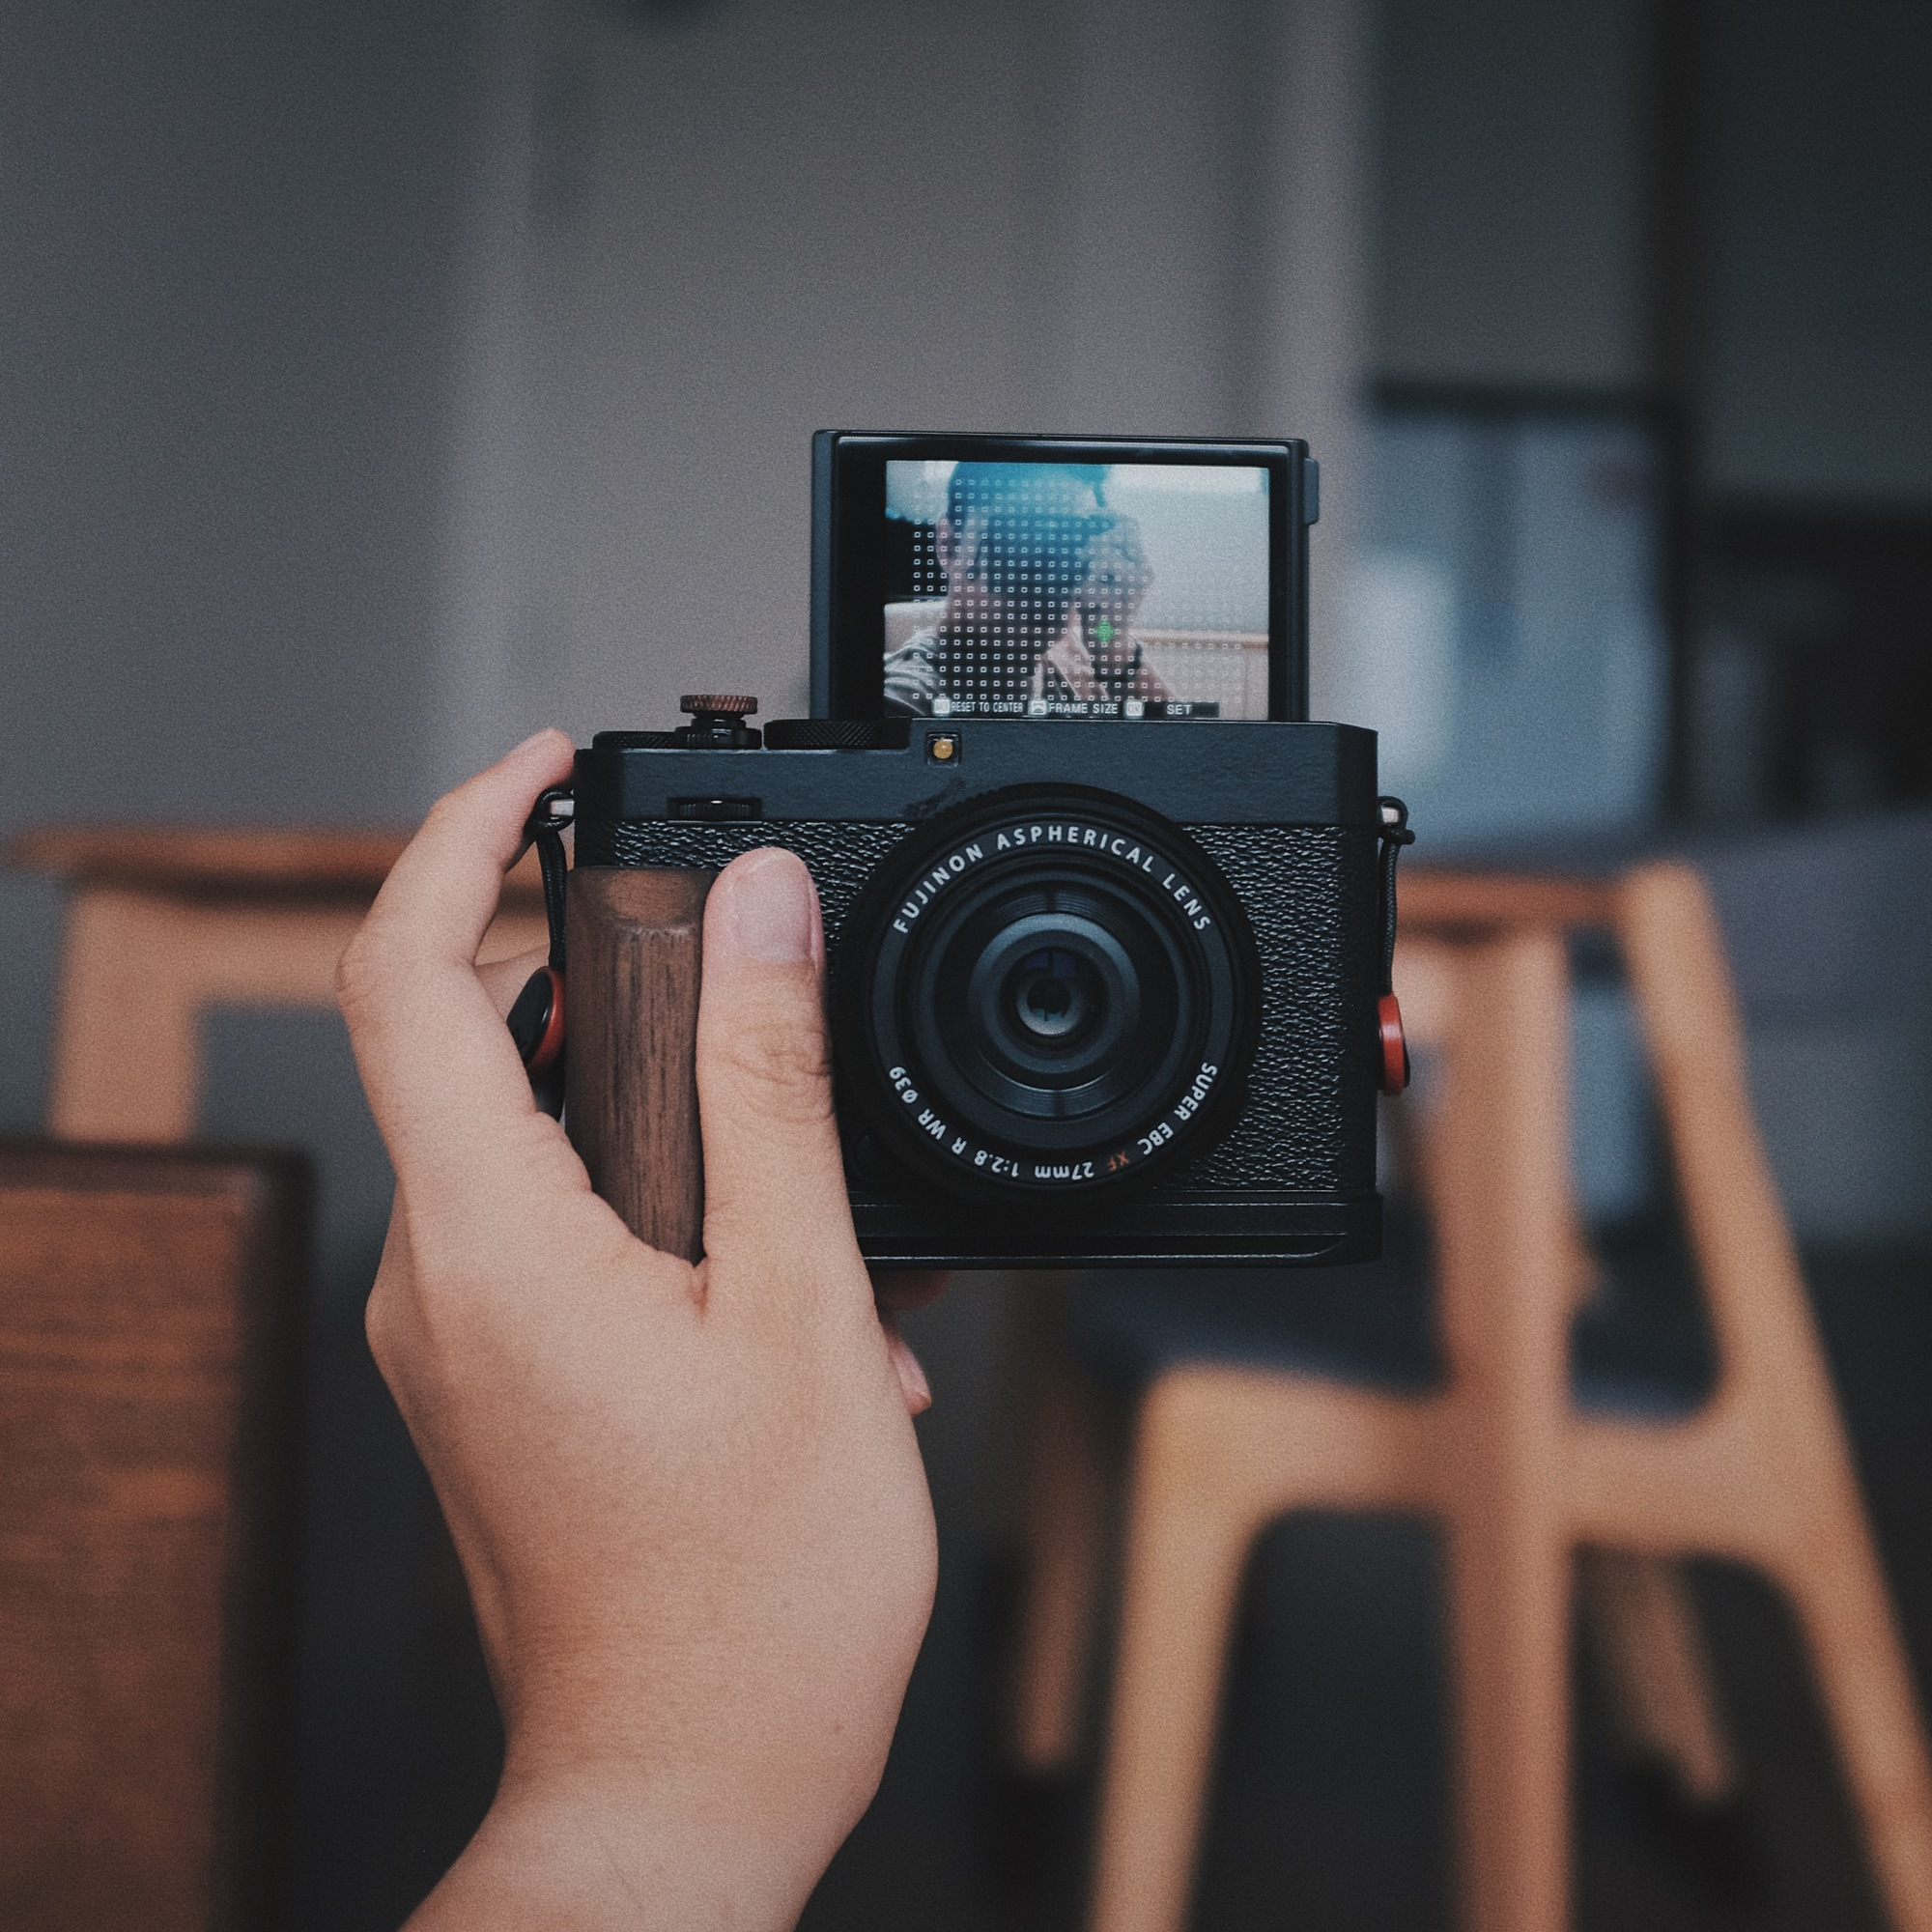
\includegraphics[width=\linewidth]{\envfinaldir/coverpic-prod.jpg}\par
            % \vskip 30pt
            \vfill

            \normalsize\rmfamily\scshape
            \copyright{} The Web Digest Project \hfill\large \envdatestr
        \end{center}
    \end{titlepage}
    % \restoregeometry
}
\newcommand{\simplehref}[1]{%
    \textcolor{blue!80!green}{\href{#1}{#1}}%
}
\renewcommand{\contentsname}{\center\Huge\sffamily\bfseries Contents\par\vskip 20pt}
\newcounter{ipartcounter}
\setcounter{ipartcounter}{0}
\newcommand{\ipart}[1]{
    % \vskip 20pt
    \clearpage
    \stepcounter{ipartcounter}
    \phantomsection
    \addcontentsline{toc}{chapter}{#1}
    % \begin{center}
    %     \Huge
    %     \sffamily\bfseries
    %     #1
    % \end{center}
    % \vskip 20pt plus 7pt
}
\newcounter{ichaptercounter}
\setcounter{ichaptercounter}{0}
\newcommand{\ichapter}[1]{
    % \vskip 20pt
    \clearpage
    \stepcounter{ichaptercounter}
    \phantomsection
    \addcontentsline{toc}{section}{\numberline{\arabic{ichaptercounter}}#1}
    \begin{center}
        \Huge
        \sffamily\bfseries
        #1
    \end{center}
    \vskip 20pt plus 7pt
}
\newcommand{\entrytitlefont}[1]{\subsection*{\raggedright\Large\sffamily\bfseries#1}}
\newcommand{\entryitemGeneric}[2]{
    % argv: title, url
    \parbox{\linewidth}{
        \entrytitlefont{#1}\par\vskip 5pt
        \footnotesize\ttfamily\mdseries
        \simplehref{#2}
    }\vskip 11pt plus 11pt minus 1pt
}
\newcommand{\entryitemGithub}[3]{
    % argv: title, url, desc
    \parbox{\linewidth}{
        \entrytitlefont{#1}\par\vskip 5pt
        \footnotesize\ttfamily\mdseries
        \simplehref{#2}\par\vskip 5pt
        \small\rmfamily\mdseries#3
    }\vskip 11pt plus 11pt minus 1pt
}
\newcommand{\entryitemAp}[3]{
    % argv: title, url, desc
    \parbox{\linewidth}{
        \entrytitlefont{#1}\par\vskip 5pt
        \footnotesize\ttfamily\mdseries
        \simplehref{#2}\par\vskip 5pt
        \small\rmfamily\mdseries#3
    }\vskip 11pt plus 11pt minus 1pt
}
\newcommand{\entryitemHackernews}[3]{
    % argv: title, hnurl, rawurl
    % \parbox{\linewidth}{
    %     \entrytitlefont{#1}\par\vskip 5pt
    %     \footnotesize\ttfamily\mdseries
    %     \simplehref{#3}\par
    %     \textcolor{black!50}{\href{#2}{#2}}
    % }\vskip 11pt plus 11pt minus 1pt
    \begin{minipage}{\linewidth}
            \entrytitlefont{#1}\par\vskip 5pt
            \footnotesize\ttfamily\mdseries
            \simplehref{#3}\par
            \textcolor{black!50}{\href{#2}{#2}}
    \end{minipage}\par\vskip 11pt plus 11pt minus 1pt
}







\begin{document}

\makeheader

\tableofcontents\clearpage




\ipart{Developers}
\ichapter{Hacker News}
\entryitemTwoLinks{Magic/tragic email links: don't make them the only option}{https://news.ycombinator.com/item?id=42627453}{https://recyclebin.zip/posts/annoyinglinks/}

\entryitemTwoLinks{Mistakes engineers make in large established codebases}{https://news.ycombinator.com/item?id=42627227}{https://www.seangoedecke.com/large-established-codebases/}

\entryitemTwoLinks{Microsoft disguises Bing as Google to fool inattentive searchers}{https://news.ycombinator.com/item?id=42626431}{https://www.pcworld.com/article/2568916/microsoft-disguises-bing-as-google-to-fool-inattentive-searchers.html}

\entryitemTwoLinks{Type 2 Diabetes and cardiovascular disease attributable to sugar beverages}{https://news.ycombinator.com/item?id=42625193}{https://www.nature.com/articles/s41591-024-03345-4}

\entryitemTwoLinks{Show HN: Tramway SDK – The Unholy Union Between Half-Life and Morrowind Engines}{https://news.ycombinator.com/item?id=42624116}{https://racenis.github.io/tram-sdk/why.html}

\entryitemTwoLinks{Show HN: HipScript – Run CUDA in the Browser with WebAssembly and WebGPU}{https://news.ycombinator.com/item?id=42623593}{https://hipscript.lights0123.com/}

\entryitemTwoLinks{Doomsday Book (2006) [pdf]}{https://news.ycombinator.com/item?id=42623144}{https://www.crisesnotes.com/content/files/2023/12/NYFRB-2006.--Doomsday-Book--Searchable.pdf}

\entryitemTwoLinks{Building Ultra Long Range Toslink}{https://news.ycombinator.com/item?id=42621766}{https://blog.benjojo.co.uk/post/sfp-experiment-ultra-long-range-toslink}

\entryitemTwoLinks{Ending our third party fact-checking program and moving to Community Notes model}{https://news.ycombinator.com/item?id=42621627}{https://about.fb.com/news/2025/01/meta-more-speech-fewer-mistakes/}

\entryitemTwoLinks{Getty Images and Shutterstock to Merge}{https://news.ycombinator.com/item?id=42621544}{https://newsroom.gettyimages.com/en/getty-images/getty-images-and-shutterstock-to-merge-creating-a-premier-visual-content-company}

\entryitemTwoLinks{Nvidia announces \$3k personal AI supercomputer called Digits}{https://news.ycombinator.com/item?id=42621332}{https://www.theverge.com/2025/1/6/24337530/nvidia-ces-digits-super-computer-ai}

\entryitemTwoLinks{First time a Blender-made production has won the Golden Globe}{https://news.ycombinator.com/item?id=42620656}{https://variety.com/2025/film/columns/flow-golden-globe-win-independent-animation-1236266805/}

\entryitemTwoLinks{Stay Gold, America}{https://news.ycombinator.com/item?id=42620278}{https://blog.codinghorror.com/}

\entryitemTwoLinks{A minimax chess engine in regular expressions}{https://news.ycombinator.com/item?id=42619652}{https://nicholas.carlini.com/writing/2025/regex-chess.html}

\entryitemTwoLinks{Nvidia's Project Digits is a 'personal AI supercomputer'}{https://news.ycombinator.com/item?id=42619139}{https://techcrunch.com/2025/01/06/nvidias-project-digits-is-a-personal-ai-computer/}

\entryitemTwoLinks{Nvidia announces next-gen RTX 5090 and RTX 5080 GPUs}{https://news.ycombinator.com/item?id=42618761}{https://www.theverge.com/2025/1/6/24337396/nvidia-rtx-5080-5090-5070-ti-5070-price-release-date}

\entryitemTwoLinks{Roman Empire's use of lead lowered IQ levels across Europe, study finds}{https://news.ycombinator.com/item?id=42618625}{https://www.theguardian.com/science/2025/jan/06/roman-empires-use-of-lead-lowered-iq-levels-across-europe-study-finds}

\entryitemTwoLinks{Zig's comptime is bonkers good}{https://news.ycombinator.com/item?id=42618130}{https://www.scottredig.com/blog/bonkers\_comptime/}

\entryitemTwoLinks{How I program with LLMs}{https://news.ycombinator.com/item?id=42617645}{https://crawshaw.io/blog/programming-with-llms}

\entryitemTwoLinks{NYC Congestion Pricing Tracker}{https://news.ycombinator.com/item?id=42616700}{https://www.congestion-pricing-tracker.com/}\ichapter{Phoronix}
\entryitemGeneric{\hskip 0pt{}Cross-Vendor Mesh Shading Being Worked On For OpenGL}{https://www.phoronix.com/news/OpenGL-GL\_EXT\_mesh\_shader}

\entryitemGeneric{\hskip 0pt{}AMD's GPUOpen HIP RT 2.5 Released With Fixes, GFX1200 RDNA4 Support}{https://www.phoronix.com/news/AMD-HIP-RT-2.5-Released}

\entryitemGeneric{\hskip 0pt{}Lenovo Officially Announces The Legion Go S Handheld With SteamOS}{https://www.phoronix.com/news/Lenovo-Legion-Go-SteamOS}

\entryitemGeneric{\hskip 0pt{}HipScript Allows NVIDIA CUDA \& AMD HIP Code To Run Within Web Browsers}{https://www.phoronix.com/news/HipScript-CUDA-HIP-Web-Browsers}

\entryitemGeneric{\hskip 0pt{}Mesa's Lavapipe Driver Now Exposes Vulkan 1.4}{https://www.phoronix.com/news/Mesa-Lavapipe-Vulkan-1.4}

\entryitemGeneric{\hskip 0pt{}GCC Goes For "libc Diversity" With Picolibc Support}{https://www.phoronix.com/news/GCC-libc-Diversity-picolibc}

\entryitemGeneric{\hskip 0pt{}Budgie 10.10 Desktop Releasing This Quarter As Wayland-Only}{https://www.phoronix.com/news/Budgie-10.10-Wayland-Only}

\entryitemGeneric{\hskip 0pt{}Device Memory "DMEM" Cgroup Support Ready For Linux 6.14 To Allow Limiting GPU vRAM}{https://www.phoronix.com/news/DMEM-cgroup-vRAM-Control}

\entryitemGeneric{\hskip 0pt{}CXL Block Device "CBD" Looking Very Promising For The Linux Kernel In 2025}{https://www.phoronix.com/news/CXL-Block-Device-Linux-v3}


\ipart{Developers~~~~(zh-Hans)}
\ichapter{Solidot}
\entryitemGeneric{\hskip 0pt{}安全公司建议不支持 Windows 11 的电脑安装 Linux}{https://www.solidot.org/story?sid=80262}

\entryitemGeneric{\hskip 0pt{}微软呼吁 Windows 10 用户换电脑}{https://www.solidot.org/story?sid=80261}

\entryitemGeneric{\hskip 0pt{}罗马帝国大规模使用铅降低了欧洲居民的智商}{https://www.solidot.org/story?sid=80260}

\entryitemGeneric{\hskip 0pt{}同样的食物为什么对每个人的影响不同}{https://www.solidot.org/story?sid=80259}

\entryitemGeneric{\hskip 0pt{}日本 2024 年平均气温创新纪录}{https://www.solidot.org/story?sid=80258}

\entryitemGeneric{\hskip 0pt{}1/10 新2型糖尿病可能是含糖饮料引起的}{https://www.solidot.org/story?sid=80257}

\entryitemGeneric{\hskip 0pt{}AMD 宣布第二代掌机芯片}{https://www.solidot.org/story?sid=80256}

\entryitemGeneric{\hskip 0pt{}美国国防部将腾讯列入中国军工公司名单}{https://www.solidot.org/story?sid=80255}

\entryitemGeneric{\hskip 0pt{}英伟达宣布 GeForce RTX 50 系列显卡}{https://www.solidot.org/story?sid=80254}

\entryitemGeneric{\hskip 0pt{}Steve Dompier 诞辰 79 周年}{https://www.solidot.org/story?sid=80253}

\entryitemGeneric{\hskip 0pt{}戴尔杀死了 XPS、Inspiron、Latitude 等 PC 品牌名称}{https://www.solidot.org/story?sid=80252}

\entryitemGeneric{\hskip 0pt{}气候危机严重破坏地球水循环}{https://www.solidot.org/story?sid=80251}

\entryitemGeneric{\hskip 0pt{}物理学家首次测量电子的量子几何}{https://www.solidot.org/story?sid=80250}

\entryitemGeneric{\hskip 0pt{}因 AI 使用上的争议期刊编辑集体辞职}{https://www.solidot.org/story?sid=80249}

\entryitemGeneric{\hskip 0pt{}更多美国电信公司披露被中国黑客入侵}{https://www.solidot.org/story?sid=80248}

\entryitemGeneric{\hskip 0pt{}新冠疫情五年之后}{https://www.solidot.org/story?sid=80247}

\entryitemGeneric{\hskip 0pt{}男子被困在在一直绕圈的 Waymo 无人驾驶出租车中}{https://www.solidot.org/story?sid=80246}

\entryitemGeneric{\hskip 0pt{}酒商用无酒精饮料吸引年轻消费者}{https://www.solidot.org/story?sid=80245}

\entryitemGeneric{\hskip 0pt{}雇主以较低的薪酬提供远程办公的灵活性}{https://www.solidot.org/story?sid=80244}

\entryitemGeneric{\hskip 0pt{}FSF 呼吁迁移出 GitHub 以抗议微软 Windows 11 对 TPM2.0 的强制性要求}{https://www.solidot.org/story?sid=80243}\ichapter{V2EX}
\entryitemGeneric{\hskip 0pt{}[macOS] 有没有 iPhone IOS 上微信双开的比较好的方案哈}{https://www.v2ex.com/t/1103359}

\entryitemGeneric{\hskip 0pt{}[Android] 小米刷机报错: update crc list failed 解决方法}{https://www.v2ex.com/t/1103358}

\entryitemGeneric{\hskip 0pt{}[宽带症候群] 网速只能跑到百兆}{https://www.v2ex.com/t/1103356}

\entryitemGeneric{\hskip 0pt{}[问与答] 入了一个 n100 小主机, 双网口, 请问目前最牛逼的玩法是什么?}{https://www.v2ex.com/t/1103355}

\entryitemGeneric{\hskip 0pt{}[问与答] 有没有使用了 GAN 技术的精巧迷你的 48V/52V POE 电源?}{https://www.v2ex.com/t/1103354}

\entryitemGeneric{\hskip 0pt{}[程序员] 现在做 ai 镜像站靠谱吗?}{https://www.v2ex.com/t/1103353}

\entryitemGeneric{\hskip 0pt{}[设计] Python 3.13 部分前端新功能与木兰对照}{https://www.v2ex.com/t/1103352}

\entryitemGeneric{\hskip 0pt{}[问与答] 请教一个车辆全损赔付问题}{https://www.v2ex.com/t/1103350}

\entryitemGeneric{\hskip 0pt{}[分享发现] [免费无水印] 告别只能使用 ios 制作备忘录的限制,一张张截图发小红书的低效工作,用这个网站在手机、电脑上 10x 效率制作备忘录}{https://www.v2ex.com/t/1103349}

\entryitemGeneric{\hskip 0pt{}[OpenAI] 分享一个目前发现低价且支持高并发的 ChatGPT API 中转站(无广)}{https://www.v2ex.com/t/1103348}

\entryitemGeneric{\hskip 0pt{}[问与答] IINA 使用问题请教}{https://www.v2ex.com/t/1103347}

\entryitemGeneric{\hskip 0pt{}[问与答] 请教关于一号多拨后的下载/上传速度异常}{https://www.v2ex.com/t/1103346}

\entryitemGeneric{\hskip 0pt{}[随想] 支持 webdav 的网盘才是好网盘}{https://www.v2ex.com/t/1103345}

\entryitemGeneric{\hskip 0pt{}[GitHub Copilot] 请问 Github Copilot 的 web search 需要怎么打开?}{https://www.v2ex.com/t/1103344}

\entryitemGeneric{\hskip 0pt{}[问与答] 求推荐 手机向 web 端推送消息服务}{https://www.v2ex.com/t/1103343}

\entryitemGeneric{\hskip 0pt{}[小米] 小米 13 pro 如何 root?}{https://www.v2ex.com/t/1103342}

\entryitemGeneric{\hskip 0pt{}[酷工作] [实习] [Tesla] [上海]信息娱乐系统前端软件开发实习生招聘}{https://www.v2ex.com/t/1103341}

\entryitemGeneric{\hskip 0pt{}[Apple] 土耳其礼品卡购买优惠渠道有哪些}{https://www.v2ex.com/t/1103340}

\entryitemGeneric{\hskip 0pt{}[React] React 不依赖第三方库怎么做到页面状态的缓存?}{https://www.v2ex.com/t/1103338}

\entryitemGeneric{\hskip 0pt{}[程序员] 2025 年了,你们用上 Virtual Threads 了吗}{https://www.v2ex.com/t/1103337}

\entryitemGeneric{\hskip 0pt{}[问与答] 请问东部地区有什么省电取暖设备吗}{https://www.v2ex.com/t/1103335}

\entryitemGeneric{\hskip 0pt{}[NAS] 不做 raid 的硬盘,真的会坏掉吗?}{https://www.v2ex.com/t/1103334}

\entryitemGeneric{\hskip 0pt{}[问与答] 品速 R200 和中兴 MC888s 选哪个?}{https://www.v2ex.com/t/1103333}

\entryitemGeneric{\hskip 0pt{}[macOS] 非程序员,有什么 mac 上比较好用的付费软件吗}{https://www.v2ex.com/t/1103331}

\entryitemGeneric{\hskip 0pt{}[上海] 对戒 购买银行金条 再找店打 是否合适}{https://www.v2ex.com/t/1103330}

\entryitemGeneric{\hskip 0pt{}[推广] 这么好用的 ai 中转 api 站点,非常稳定,欢迎使用}{https://www.v2ex.com/t/1103329}

\entryitemGeneric{\hskip 0pt{}[Apple] iOS 18.2.1 相機鏡頭切換問題}{https://www.v2ex.com/t/1103328}

\entryitemGeneric{\hskip 0pt{}[分享创造] 从 4.3 到成功上架,分享过去一年独开的探索之路(踩坑经历)}{https://www.v2ex.com/t/1103327}

\entryitemGeneric{\hskip 0pt{}[程序员] 求推荐学习英语的 APP}{https://www.v2ex.com/t/1103326}

\entryitemGeneric{\hskip 0pt{}[问与答] 魂签,这个签到插件作者放弃了么,怎么 Github 账号也没了}{https://www.v2ex.com/t/1103324}

\entryitemGeneric{\hskip 0pt{}[职场话题] 找外企工作会要求托福/雅思成绩在有效期内吗?}{https://www.v2ex.com/t/1103323}

\entryitemGeneric{\hskip 0pt{}[推广] 腾爱优 小程序上线了}{https://www.v2ex.com/t/1103322}

\entryitemGeneric{\hskip 0pt{}[Local LLM] 英伟达个人 AI 超算 Project Digits 发布 起售价 3000 美元}{https://www.v2ex.com/t/1103321}

\entryitemGeneric{\hskip 0pt{}[Windows] windows 7 平台有没有软件可以像 ios 里的 share 一样}{https://www.v2ex.com/t/1103320}

\entryitemGeneric{\hskip 0pt{}[数学] 闭区间连续函数有界的证明为什么都要用到数列?}{https://www.v2ex.com/t/1103316}

\entryitemGeneric{\hskip 0pt{}[Python] Windows 新版本怎么实现截图}{https://www.v2ex.com/t/1103314}

\entryitemGeneric{\hskip 0pt{}[问与答] [请教] 如何在日本买 5090 回国}{https://www.v2ex.com/t/1103313}

\entryitemGeneric{\hskip 0pt{}[分享创造] 分享自己开发的看图猜电影小程序}{https://www.v2ex.com/t/1103312}

\entryitemGeneric{\hskip 0pt{}[互联网] 求推荐类似 V2EX 的开源论坛!}{https://www.v2ex.com/t/1103310}

\entryitemGeneric{\hskip 0pt{}[程序员] CodeWithMosh 怎么样? 29 刀一个月的视频课}{https://www.v2ex.com/t/1103309}

\entryitemGeneric{\hskip 0pt{}[Docker] bitnami 现在开始收费了 有点没理解}{https://www.v2ex.com/t/1103308}

\entryitemGeneric{\hskip 0pt{}[玩家国度] ROG NUC 2025 发布了, 5080 强势登场}{https://www.v2ex.com/t/1103307}

\entryitemGeneric{\hskip 0pt{}[生活] 我丢! 29 岁高血压}{https://www.v2ex.com/t/1103306}

\entryitemGeneric{\hskip 0pt{}[酷工作] 发个私活,加固 rust 语言打包的 exe 程序,预算 1k}{https://www.v2ex.com/t/1103305}

\entryitemGeneric{\hskip 0pt{}[Java] 关于分库分表的一点疑惑}{https://www.v2ex.com/t/1103304}

\entryitemGeneric{\hskip 0pt{}[问与答] cursor 写出来的项目有版权吗,版权归属使用 cursor 的人吗}{https://www.v2ex.com/t/1103303}

\entryitemGeneric{\hskip 0pt{}[程序员] pycharm 自动 import 好抽象}{https://www.v2ex.com/t/1103302}

\entryitemGeneric{\hskip 0pt{}[生活] 彩礼超 10 万就要反对}{https://www.v2ex.com/t/1103301}

\entryitemGeneric{\hskip 0pt{}[程序员] 副业的一些经验分享: youtube / 云手机}{https://www.v2ex.com/t/1103300}

\entryitemGeneric{\hskip 0pt{}[职场话题] 请问下简历花了怎么办?或者说简历上没亮点怎么办?}{https://www.v2ex.com/t/1103299}


\ipart{Generic News}
\ichapter{AP News}
\entryitemWithDescription{\hskip 0pt{}Peter Yarrow of folk-music trio Peter, Paul and Mary dies at 86}{https://apnews.com/article/767c223e40c243199b0d0875e29a5efc}{}

\entryitemWithDescription{\hskip 0pt{}Trump says he will change the name of the Gulf of Mexico}{https://apnews.com/article/bc438f4feca1234475a1adef99344da7}{}

\entryitemWithDescription{\hskip 0pt{}Donald Trump Jr. arrives in Greenland with a message from his dad: `We're going to treat you well'}{https://apnews.com/article/56bc01f1d3431c035b22ad6564579938}{}

\entryitemWithDescription{\hskip 0pt{}NASA proposes cheaper, quicker way to get Mars rocks and soil to Earth}{https://apnews.com/article/6b6028cd2866f41f39864717f70e979d}{}

\entryitemWithDescription{\hskip 0pt{}2 bodies are found in the landing gear of JetBlue plane at Florida airport}{https://apnews.com/article/67485cd731e0933011b61cda112c6f38}{}

\entryitemWithDescription{\hskip 0pt{}Elk on a shelf: Colorado wildlife officials rescue elk tangled in rope on ice climbing route}{https://apnews.com/article/76ac11829a4f612da2e020a56481d7e1}{}

\entryitemWithDescription{\hskip 0pt{}San Diego State University frat members charged after pledge set on fire at party, prosecutors say}{https://apnews.com/article/140f97800826c4e08f586f37f60c778c}{}

\entryitemWithDescription{\hskip 0pt{}2 sons of Mexican cartel leader `El Chapo' are in plea negotiations with US, attorneys say}{https://apnews.com/article/da8c7f5df283255c389a527c26193b63}{}

\entryitemWithDescription{\hskip 0pt{}Biggest Nvidia takeaways from Jensen Huang's CES 2025 keynote}{https://apnews.com/article/fadab7fc10c1a3e306c0a16448559ad8}{}

\entryitemWithDescription{\hskip 0pt{}Suspect in NYC subway burning told police `that's me' when shown video, transcript says}{https://apnews.com/article/94a5c2af2ac380a4ab991a5a40ab068e}{}

\entryitemWithDescription{\hskip 0pt{}Donald Trump Jr. will visit Greenland as his father muses anew about the US taking control of it}{https://apnews.com/article/7a235a1e756c48ffdb4a3158ced35514}{}

\entryitemWithDescription{\hskip 0pt{}Jaguars fire coach Doug Pederson, keep GM Trent Baalke after `best team assembled' wins just 4 games}{https://apnews.com/article/20f47f397e7885c8dd0fce10ac283076}{}

\entryitemWithDescription{\hskip 0pt{}Inside the Golden Globes: What you didn't see on television}{https://apnews.com/article/6856384ad8702326885542d9585d20c9}{}\ichapter{Reuters}
\entryitemWithDescription{\hskip 0pt{}Brazil's Lula swaps presidential spokesperson for former campaign advisor}{https://www.reuters.com/world/americas/brazils-lula-swaps-presidential-spokesperson-former-campaign-advisor-2025-01-07/}{Brazilian President Luiz Inacio Lula da Silva decided to replace his presidential spokesperson Paulo Pimenta in favor for Sidonio Palmeira, a former advisor who worked with Lula during his successful 2022 presidential...}

\entryitemWithDescription{\hskip 0pt{}Harris to travel to Singapore, Bahrain and Germany before leaving office}{https://www.reuters.com/world/harris-travel-singapore-bahrain-germany-before-leaving-office-2025-01-07/}{U.S. Vice President Kamala Harris will travel to Europe, the Middle East and Asia from Jan. 13 through Jan. 17, the White House said on...}

\entryitemWithDescription{\hskip 0pt{}Trump says he sympathizes with Russia's opposition to NATO membership for Ukraine}{https://www.reuters.com/world/trump-says-he-sympathizes-with-russias-opposition-nato-membership-ukraine-2025-01-07/}{President-elect Donald Trump said on Tuesday he sympathized with the Russian position that Ukraine should not be part of NATO, and he lamented that he will not meet Russian President Vladimir Putin before his...}

\entryitemWithDescription{\hskip 0pt{}What Trump said about Canada, Mexico, NATO and Gaza hostages at news conference}{https://www.reuters.com/world/us/what-trump-said-about-canada-mexico-nato-gaza-hostages-news-conference-2025-01-07/}{Republican U.S. President-elect Donald Trump held a press conference on Tuesday and spoke about a range of issues including NATO, Israeli hostages in Gaza, his wish for the U.S. to buy Greenland and take control of the Panama...}

\entryitemWithDescription{\hskip 0pt{}British minister says Musk knows 'absolutely nothing' about child rape scandals}{https://www.reuters.com/world/uk/british-minister-says-musk-knows-absolutely-nothing-about-child-rape-scandals-2025-01-07/}{A British minister who Elon Musk has described as a "rape genocide apologist" said on Tuesday the U.S. billionaire knew "absolutely nothing" about the child sexual abuse scandals he has recently been commenting...}

\entryitemWithDescription{\hskip 0pt{}Two men fatally injured after shooting at company in southern Germany, police say}{https://www.reuters.com/markets/europe/two-men-fatally-injured-after-shooting-company-southern-germany-police-say-2025-01-07/}{Two men were fatally injured on Tuesday evening after shots were fired at a company in Bad Friedrichshall in the state of Baden-Wuerttemberg in southern Germany, local police said in a...}

\entryitemWithDescription{\hskip 0pt{}Trudeau rejects Trump's idea of forcing Canada to become a US state}{https://www.reuters.com/world/americas/canada-rejects-trumps-comments-about-possible-use-economic-force-2025-01-07/}{Canadian Prime Minister Justin Trudeau on Tuesday dismissed a suggestion by U.S. President-elect Donald Trump that he might use "economic force" to make Canada the 51st U.S...}

\entryitemWithDescription{\hskip 0pt{}Turkey says it will mount offensive against Kurdish YPG if demands not met}{https://www.reuters.com/world/middle-east/turkey-says-it-will-mount-offensive-against-kurdish-ypg-if-group-does-not-meet-2025-01-07/}{Turkey will carry out a cross-border offensive into northeastern Syria against the Kurdish YPG militia if the group does not meet Ankara\textquotesingle s demands, Foreign Minister Hakan Fidan said on Tuesday, while adding that Syria...}

\entryitemWithDescription{\hskip 0pt{}Can Trump buy Greenland?}{https://www.reuters.com/world/can-trump-buy-greenland-2025-01-07/}{U.S. President-elect Donald Trump says he wants to make Greenland a part of the United States, renewing an interest first expressed in 2019 when he offered to buy the sprawling Arctic island from Denmark - and was...}

\entryitemWithDescription{\hskip 0pt{}Germany pushing for EU to relax sanctions on Syria, sources say}{https://www.reuters.com/world/europe/germany-pushing-eu-relax-sanctions-syria-ft-reports-2025-01-07/}{Germany is leading European Union discussions on easing sanctions imposed on the Syrian government of toppled President Bashar al-Assad and aiding the country\textquotesingle s population, foreign ministry sources said on...}

\entryitemWithDescription{\hskip 0pt{}Trump Middle East envoy predicts 'good things' to announce on Gaza hostages before inauguration}{https://www.reuters.com/world/middle-east/trump-middle-east-envoy-predicts-good-things-announce-gaza-hostages-before-2025-01-07/}{President-elect Donald Trump\textquotesingle s Middle East envoy Steve Witkoff said on Tuesday he hopes to have good things to report about hostages held by Hamas in Gaza by the time Trump is sworn in as U.S. president on Jan...}

\entryitemWithDescription{\hskip 0pt{}Israel says no foreign courts have warrants issued against reservists}{https://www.reuters.com/world/middle-east/israel-says-no-foreign-courts-have-warrants-issued-against-reservists-2025-01-07/}{Israel said on Tuesday pressure groups were pushing foreign courts to take action against Israelis over alleged war crimes in Gaza but described the actions as "propaganda activity" and said no warrants had been...}

\entryitemWithDescription{\hskip 0pt{}Trump won't rule out force to take Panama Canal, Greenland}{https://www.reuters.com/world/trump-wont-rule-out-military-economic-action-he-seeks-control-panama-canal-2025-01-07/}{U.S. President-elect Donald Trump refused on Tuesday to rule out using military or economic action to pursue acquisition of the Panama Canal and Greenland, part of a broader expansionist agenda he has promoted since winning the Nov. 5...}






\clearpage
\leavevmode\vfill
\footnotesize

Copyright \copyright{} 2023-2025 Neruthes and other contributors.

This document is published with CC BY-NC-ND 4.0 license.

The entries listed in this newsletter may be copyrighted by their respective creators.

This newsletter is generated by the Web Digest project.

The newsletters are also delivered via Telegram channel \CJKunderline{\href{https://t.me/webdigestchannel}{https://t.me/webdigestchannel}}.\\
RSS feed is available at \CJKunderline{\href{https://webdigest.pages.dev/rss.xml}{https://webdigest.pages.dev/rss.xml}}.

This newsletter is available in PDF at
\CJKunderline{\href{https://webdigest.pages.dev/}{https://webdigest.pages.dev/}}.

The source code being used to generate this newsletter is available at\\
\CJKunderline{\href{https://github.com/neruthes/webdigest}{https://github.com/neruthes/webdigest}}.

This newsletter is also available in
\CJKunderline{\href{http://webdigest.pages.dev/readhtml/\envyear/WebDigest-20250108.html}{HTML}} and
\CJKunderline{\href{https://github.com/neruthes/webdigest/blob/master/markdown/\envyear/WebDigest-20250108.md}{Markdown}}.


\coverpic{https://unsplash.com/photos/aerial-view-of-boats-docked-in-a-harbor-\_iTeUl9U8kA}{Willian Justen de Vasconcellos}


\end{document}
